

 
\documentclass[12pt]{article}
 
\usepackage[margin=1in]{geometry} 
\usepackage{amsmath,amsthm,amssymb}
\usepackage{graphicx}
 
\begin{document}
 

 
\title{Resultados Tarea 4}
\author{Benjamin Leon\\
Metodos Computacionales tarea \# 4} 
\maketitle


\section{Ecuaciones diferenciales Ordinarias (ODE)}
\begin{centering}
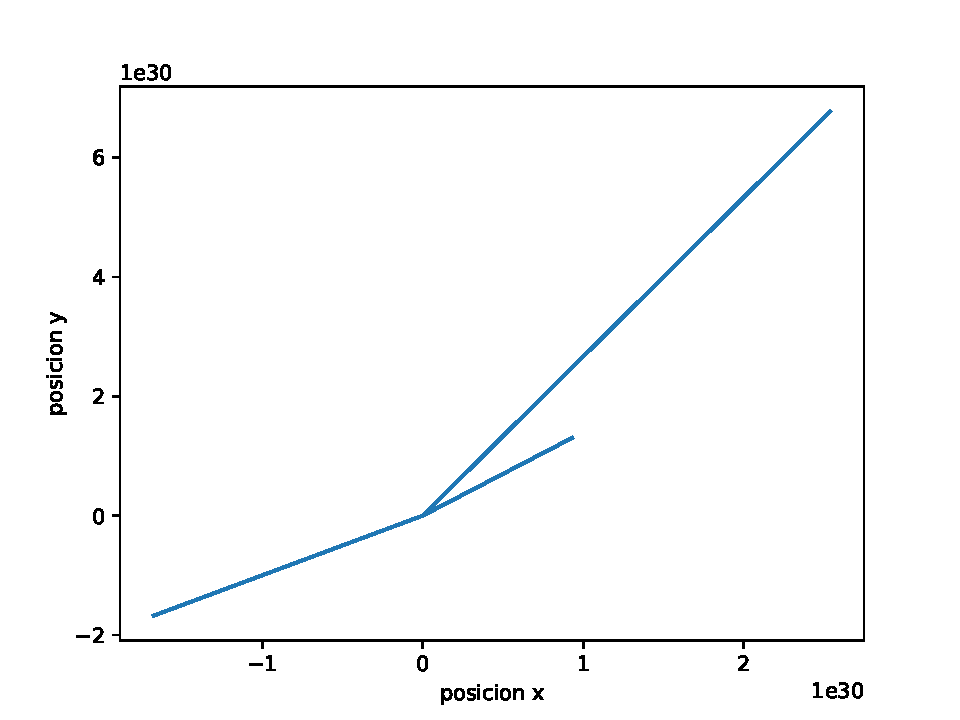
\includegraphics[width=0.75\textwidth]{grafsODE.pdf}

Deberia mostrar las diferentes trayectorias seg\'un el angulo de lanzamiento, pero por alg\'un error muestra lineas rectas

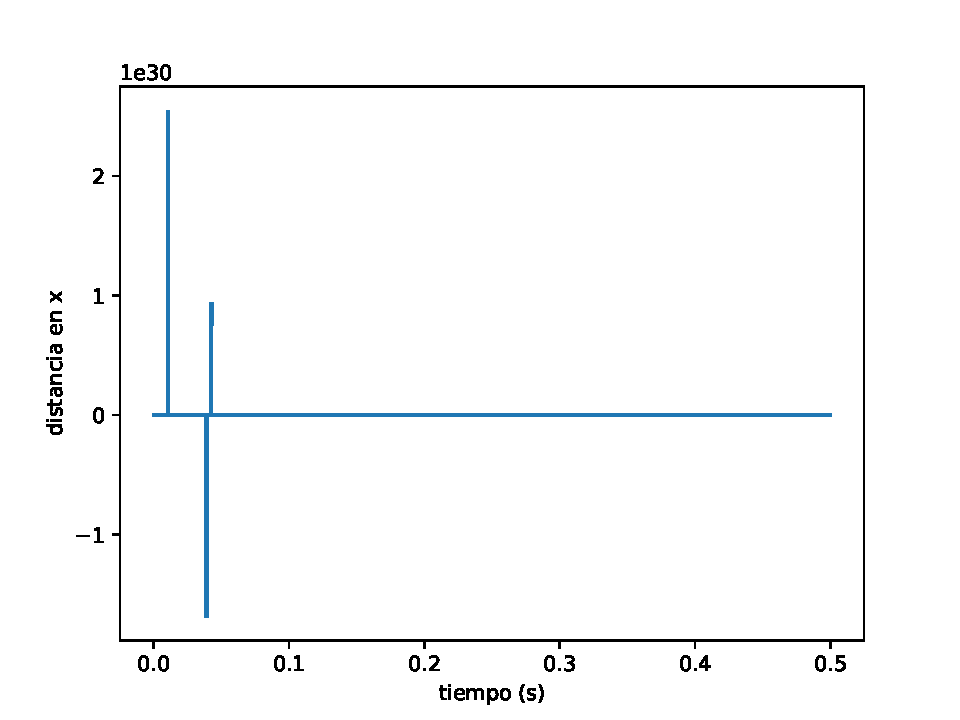
\includegraphics[width=0.75\textwidth]{grafsODE2.pdf}

Muestra la posicion en "x" con respecto al tiempo "t"
\end{centering}


\section{Ecuaciones diferenciales Parciales(PDE)}
\begin{centering}
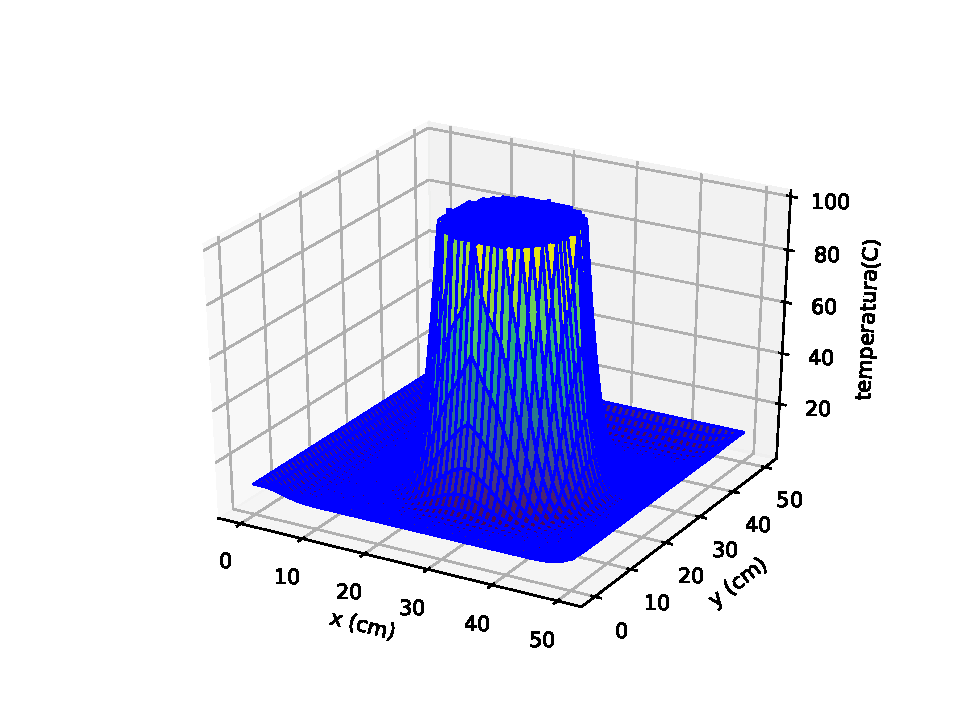
\includegraphics[width=0.75\textwidth]{3d2.pdf}
\\
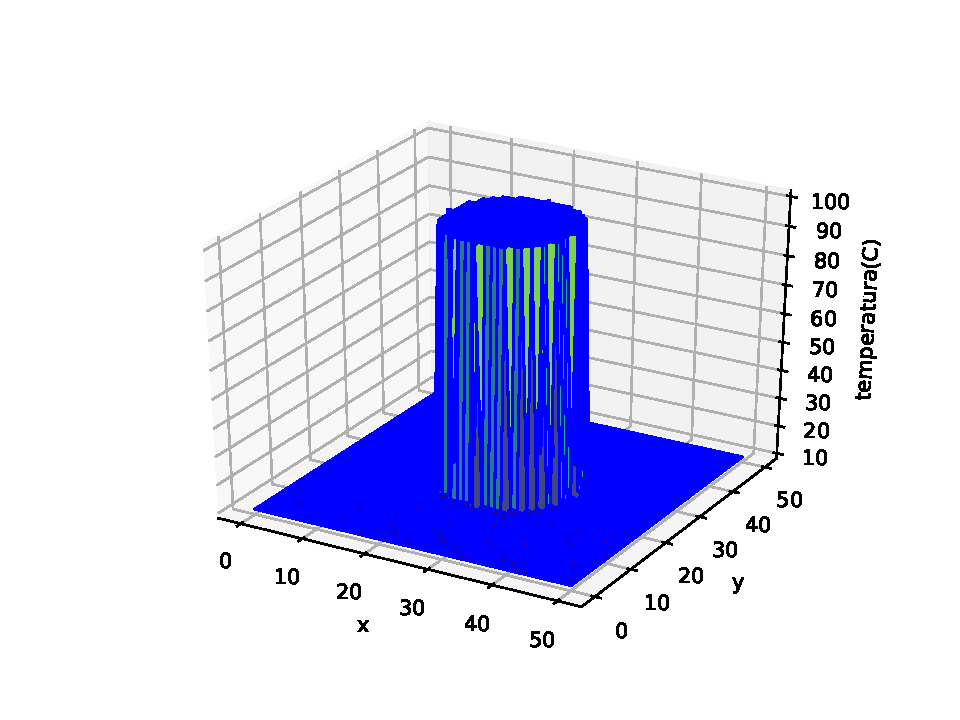
\includegraphics[width=0.75\textwidth]{3d3.pdf}

Se deberian ver las tempratura despues de mil pasos pero solo se ven las temperaturas iniciales
\end{centering}

 
\end{document}
